% Carbu-Rat - Rapido & Razmo : 10-minute project presentation (Beamer, 16:9)
\documentclass[aspectratio=169,11pt]{beamer}

\usepackage[T1]{fontenc}
\usepackage[utf8]{inputenc}
\usepackage[sfdefault,scaled=.95]{FiraSans}
\usepackage[scaled=.95]{inconsolata}
\usepackage{textcomp}
\usepackage{booktabs}
\usepackage{array}
\usepackage{tikz}
\usetikzlibrary{positioning,arrows.meta,shapes.geometric,calc,fit,backgrounds}
\usepackage{pgfplots}
\pgfplotsset{compat=1.17}
\usepackage{fontawesome5}
\usepackage{appendixnumberbeamer}

% ---------- Colours (taken from the Ratz logo and the two characters) ----------
\definecolor{ratzpurple}{HTML}{3F1F6E}
\definecolor{ratzyellow}{HTML}{F5C518}
\definecolor{ratzorange}{HTML}{F07A3A}
\definecolor{rapidored}{HTML}{B71C1C}
\definecolor{razmoblue}{HTML}{3B7DD8}
\definecolor{ink}{HTML}{222222}
\definecolor{soft}{HTML}{6B6B7B}
\definecolor{paper}{HTML}{F6F4FA}
\definecolor{okgreen}{HTML}{2E7D32}

% ---------- Minimal custom theme ----------
\setbeamertemplate{navigation symbols}{}
\setbeamercolor{background canvas}{bg=white}
\setbeamercolor{normal text}{fg=ink}
\setbeamercolor{structure}{fg=ratzpurple}
\setbeamercolor{alerted text}{fg=rapidored}
\setbeamerfont{frametitle}{size=\Large,series=\bfseries}
\setbeamertemplate{frametitle}{%
  \vskip6pt\usebeamerfont{frametitle}\color{ratzpurple}\insertframetitle\par
  \vskip2pt{\color{ratzyellow}\rule{2.2cm}{2.5pt}}\vskip2pt}
\setbeamertemplate{footline}{%
  \hbox to\paperwidth{\hskip12pt\color{soft}\tiny Carbu-Rat \textperiodcentered{} Rapido \& Razmo\hfill\insertframenumber\,/\,\inserttotalframenumber\hskip12pt}\vskip6pt}
\setbeamertemplate{itemize item}{\color{ratzorange}\raisebox{1pt}{\scriptsize$\blacktriangleright$}}
\setbeamertemplate{itemize subitem}{\color{soft}--}
\setlength{\leftmargini}{1.2em}

\newcommand{\cmd}[1]{\leavevmode{\ttfamily\color{ratzpurple}#1}}
\newcommand{\rapido}{{\color{rapidored}\bfseries Rapido}}
\newcommand{\razmo}{{\color{razmoblue}\bfseries Razmo}}
\newcommand{\eur}{\,\texteuro}

\tikzset{
  box/.style={draw=#1, fill=#1!8, rounded corners=3pt, line width=0.8pt, align=center, font=\scriptsize, inner sep=4pt},
  box/.default=ratzpurple,
  arr/.style={-{Stealth[length=5pt]}, line width=0.7pt, color=soft},
  lbl/.style={font=\tiny, color=soft, fill=white, inner sep=1pt}
}

\title{Carbu-Rat}
\subtitle{Rapido \& Razmo, the fuel-price rats}
\author{Josh E. SOUSSAN}
\date{October 2026}

\begin{document}

% =====================================================================
% 1. Title
\begin{frame}[plain]
  \begin{tikzpicture}[remember picture,overlay]
    \fill[paper] (current page.north west) rectangle (current page.south east);
    \fill[ratzpurple] (current page.south west) rectangle ([yshift=0.5cm]current page.south east);
    \node[anchor=south west, inner sep=0] at ([xshift=0.3cm,yshift=0.6cm]current page.south west)
      {
\includegraphics[height=5.4cm]{img/rapido.png}};
    \node[anchor=south east, inner sep=0] at ([xshift=-0.15cm,yshift=0.6cm]current page.south east)
      {
\includegraphics[height=3.0cm]{img/razmo.png}};
    \node[anchor=north] at ([yshift=-0.3cm,xshift=0.3cm]current page.north)
      {
\includegraphics[height=1.9cm]{img/ratz_fr_logo.png}};
    \node[align=center, text width=7.4cm] at ([yshift=-0.55cm,xshift=0.3cm]current page.center) {%
      {\fontsize{34}{36}\selectfont\bfseries\color{ratzpurple} Carbu-Rat}\\[4pt]
      {\large\color{ink} Rapido \& Razmo,\\ the fuel-price rats}\\[8pt]
      {\small\color{soft} A fuel-price assistant and threshold alerts\\ on Telegram, built on n8n}\\[10pt]
      {\normalsize\bfseries Josh E. SOUSSAN}\\[1pt]{\small\color{soft}October 2026 \textperiodcentered{} Level 3}};
    \node[anchor=south, text=white, font=\tiny] at (current page.south)
      {\raisebox{1.5pt}{n8n \textperiodcentered{} Telegram $\times$2 \textperiodcentered{} NanoGPT \textperiodcentered{} n8n Data Tables \textperiodcentered{} Fuel-price open data \textperiodcentered{} French geocoding API}};
  \end{tikzpicture}
\end{frame}

% =====================================================================
% 2. The need
\begin{frame}{The need}
  \begin{columns}[c]
    \begin{column}{0.42\textwidth}
      \centering
      {\fontsize{54}{56}\selectfont\bfseries\color{rapidored} 15--20\,c}\\[2pt]
      {\large\color{ink} more per litre}\\[2pt]
      {\small\color{soft} depending on the station you pick,\\ in the same area, on the same day}
    \end{column}
    \begin{column}{0.55\textwidth}
      {\large\bfseries\color{ratzpurple}Drivers in France check fuel prices on a comparison website by hand, when they remember to, and never know when prices drop.}
      \vspace{8pt}
      \begin{itemize}\setlength{\itemsep}{4pt}
        \item Prices change \textbf{every day}.
      \end{itemize}
      \vspace{10pt}
      \begin{beamercolorbox}[rounded=true,sep=8pt]{block body}
        \small\textbf{Goal:} answer ``where do I fill up?'' in seconds, and warn me
        \emph{once} when my target price is reached.
      \end{beamercolorbox}
    \end{column}
  \end{columns}
\end{frame}

% =====================================================================
% 3. Meet the duo
\begin{frame}{Meet the duo: two rats, two bots}
  \begin{columns}[T,onlytextwidth]
    \begin{column}{0.49\textwidth}
      \begin{minipage}[t]{2.6cm}\vspace{0pt}\centering
        
\includegraphics[height=4.2cm]{img/rapido.png}
      \end{minipage}\hfill
      \begin{minipage}[t]{\dimexpr\linewidth-2.8cm}\vspace{0pt}
        {\Large\rapido}\\{\scriptsize\color{soft}@rapido\_carbu\_bot\\\textbf{the one you ask}}\\[5pt]
        \footnotesize
        \begin{itemize}\setlength{\itemsep}{3pt}
          \item \cmd{/plein Créteil gazole}:\\ top 5 cheapest pumps nearby
          \item Free text, answered by an \textbf{AI agent}
          \item Small, fast, short sentences
          \item \textbf{Pull}: only ever answers
        \end{itemize}
      \end{minipage}
    \end{column}
    \begin{column}{0.49\textwidth}
      \begin{minipage}[t]{3.2cm}\vspace{14pt}\centering
        
\includegraphics[width=3.2cm]{img/razmo.png}
      \end{minipage}\hfill
      \begin{minipage}[t]{\dimexpr\linewidth-3.4cm}\vspace{0pt}
        {\Large\razmo}\\{\scriptsize\color{soft}@razmo\_carbu\_bot\\\textbf{the one who watches}}\\[5pt]
        \footnotesize
        \begin{itemize}\setlength{\itemsep}{3pt}
          \item \cmd{/alerte gazole 1,65 Créteil}
          \item Checks the pumps \textbf{twice a day}
          \item Big, calm, speaks of himself in the 3rd person
          \item \textbf{Push}: the only one who writes first
        \end{itemize}
      \end{minipage}
    \end{column}
  \end{columns}
  \vspace{6pt}
  \centering\scriptsize\color{soft}
  Two bots, so the user can \textbf{mute the alerts without losing the assistant}.\\ A nod to the cartoon \emph{Ratz}; the lines are our own.
\end{frame}

% =====================================================================
% 4. Architecture
\begin{frame}{Architecture: five workflows, one journey}
  \centering
  \resizebox{\linewidth}{!}{%
  \begin{tikzpicture}
    % entry points (left column)
    \node[box=rapidored, minimum width=2.4cm] (tgA) at (0,1.8) {\faTelegram\ Rapido\\[-1pt]\tiny Telegram Trigger};
    \node[box=soft, minimum width=2.4cm] (sch) at (0,0.2) {\faClock\ 07:00 \& 18:00\\[-1pt]\tiny Schedule + Manual};
    \node[box=razmoblue, minimum width=2.4cm] (tgZ) at (0,-1.4) {\faTelegram\ Razmo\\[-1pt]\tiny Telegram Trigger};
    % workflows
    \node[box=rapidored, minimum width=2.9cm] (wf1) at (3.7,1.8) {\textbf{WF1 Rapido}\\[-1pt]\tiny router, AI agent, deep link};
    \node[box=ratzorange, minimum width=2.9cm] (wf3) at (3.7,0.2) {\textbf{WF3 Price sweep}\\[-1pt]\tiny loop, hysteresis, LLM line};
    \node[box=razmoblue, minimum width=2.9cm] (wf4) at (3.7,-1.4) {\textbf{WF4 Razmo}\\[-1pt]\tiny commands, validation};
    % shared core
    \node[box=okgreen, minimum width=3.0cm] (wf2) at (8.9,1.8) {\textbf{WF2 Find stations}\\[-1pt]\tiny sub-workflow, zero AI};
    \node[box=ratzpurple, minimum width=3.0cm] (dt) at (8.9,-1.4)
      {\faDatabase\ \textbf{Data Tables}\\[-1pt]\tiny alerts \textperiodcentered{} price\_history \textperiodcentered{} config};
    % external services
    \node[box=soft, minimum width=2.7cm] (geo) at (13.6,2.5) {Geocoding API\\[-1pt]\tiny keyless};
    \node[box=soft, minimum width=2.7cm] (fuel) at (13.6,1.1) {Fuel-price open data\\[-1pt]\tiny keyless};
    \node[box=soft, minimum width=2.7cm, text width=2.5cm] (llm) at (13.6,-0.3) {NanoGPT LLM\\[-1pt]\tiny used by the WF1 agent\\[-2pt]and the WF3 punchline};
    % error workflow
    \node[box=rapidored, fill=rapidored!10, minimum width=13.8cm] (wf5) at (6.8,-2.75)
      {\textbf{WF5 Error}\quad\tiny any crash in WF1--WF4 $\rightarrow$ Telegram message to the owner, through Razmo};

    \draw[arr] (tgA) -- node[lbl, above]{chat\_id + text} (wf1);
    \draw[arr] (sch) -- node[lbl, above]{tick} (wf3);
    \draw[arr] (tgZ) -- node[lbl, above]{chat\_id + text} (wf4);
    \draw[arr] (wf1) -- node[lbl, above]{place, fuel / top 5} (wf2);
    \draw[arr] (wf3.east) -- node[lbl, above, sloped]{place, fuel} (wf2.south west);
    \draw[arr] (wf3.east) -- node[lbl, below, sloped]{rows / armed=false} (dt.north west);
    \draw[arr] (wf3.east) -- node[lbl, above, pos=0.78]{1 sentence} (llm.west);
    \draw[arr] (wf4) -- node[lbl, above]{alert record} (dt);
    \draw[arr] (wf4) -- node[lbl, right]{/sweep} (wf3);
    \draw[arr] (wf2.east) -- node[lbl, above, sloped]{place} (geo.west);
    \draw[arr] (wf2.east) -- node[lbl, below, sloped]{lat, lon, fuel} (fuel.west);
    \draw[arr, dashed, rapidored] (tgA.west) .. controls +(-2.2,0) and +(-2.2,0) .. node[lbl, pos=0.5, fill=white, align=center]{deep link\\a\_gazole\_222\_94000} (tgZ.west);
  \end{tikzpicture}}
  \vspace{2pt}
  {\scriptsize\color{soft}\textbf{Level 3.} Cut line, first dropped: \cmd{/tendance} $\rightarrow$ deep link $\rightarrow$ LLM punchline $\rightarrow$ agent memory. Never cut: \cmd{/plein}, \cmd{/alerte}, sweep + hysteresis, error workflow.}
\end{frame}

% =====================================================================
% 9. Hysteresis
\begin{frame}{Hysteresis: never the same ping twice}
  \begin{columns}[c]
    \begin{column}{0.58\textwidth}
      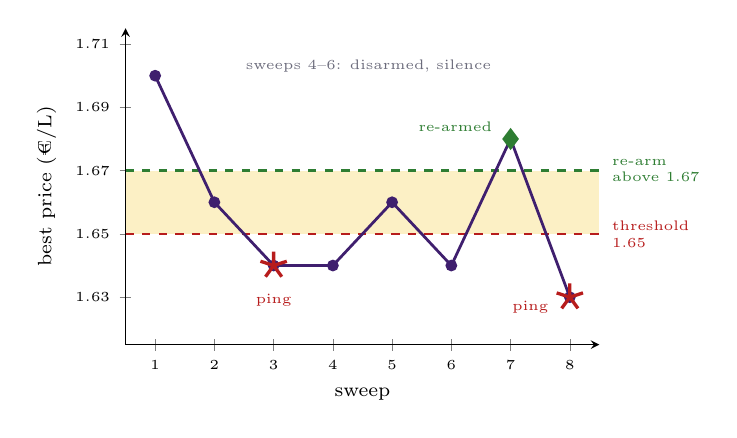
\begin{tikzpicture}
        \begin{axis}[
          width=7.6cm, height=5.6cm, clip=false,
          xmin=0.5, xmax=8.5, ymin=1.615, ymax=1.715,
          xtick={1,...,8}, xlabel={\scriptsize sweep}, ylabel={\scriptsize best price (\texteuro/L)},
          ytick={1.63,1.65,1.67,1.69,1.71},
          yticklabel style={/pgf/number format/.cd,fixed,precision=2,fixed zerofill},
          tick label style={font=\tiny}, axis lines=left, grid=none,
          every axis plot/.append style={line width=1pt}]
          \fill[ratzyellow!25] (axis cs:0.5,1.65) rectangle (axis cs:8.5,1.67);
          \addplot[rapidored, dashed, domain=0.5:8.5, samples=2] {1.65};
          \addplot[okgreen, dashed, domain=0.5:8.5, samples=2] {1.67};
          \node[font=\tiny, rapidored, anchor=west, align=left] at (axis cs:8.55,1.65) {threshold\\1.65};
          \node[font=\tiny, okgreen, anchor=west, align=left] at (axis cs:8.55,1.67) {re-arm\\above 1.67};
          \addplot[ratzpurple, mark=*, mark size=1.6pt] coordinates {(1,1.70)(2,1.66)(3,1.64)(4,1.64)(5,1.66)(6,1.64)(7,1.68)(8,1.63)};
          \addplot[only marks, mark=star, mark size=5pt, rapidored, line width=1.2pt] coordinates {(3,1.64)(8,1.63)};
          \addplot[only marks, mark=diamond*, mark size=3.2pt, okgreen] coordinates {(7,1.68)};
          \node[font=\tiny, rapidored] at (axis cs:3,1.629) {ping};
          \node[font=\tiny, rapidored, anchor=east] at (axis cs:7.8,1.627) {ping};
          \node[font=\tiny, okgreen, anchor=east] at (axis cs:6.85,1.684) {re-armed};
          \node[font=\tiny, soft, align=center] at (axis cs:4.6,1.703) {sweeps 4--6: disarmed, silence};
        \end{axis}
      \end{tikzpicture}
    \end{column}
    \begin{column}{0.40\textwidth}
      \small
      Each alert has an \texttt{armed} flag.\\[6pt]
      {\color{rapidored}\faBell}\ \textbf{fire} if price $\leq$ threshold \textbf{and} armed\\
      \hspace*{1.3em}{\scriptsize\color{soft}then armed = false}\\[4pt]
      {\color{okgreen}\faRedo}\ \textbf{re-arm} if price $>$ threshold + 2\,c\\
      \hspace*{1.3em}{\scriptsize\color{soft}and the alert is disarmed}\\[4pt]
      {\color{soft}\faMinus}\ otherwise \textbf{skip}\\[10pt]
      \begin{beamercolorbox}[rounded=true,sep=6pt]{block body}
        \scriptsize The 2-cent margin works like a thermostat: a price wobbling around the threshold does \textbf{not} spam the user.
      \end{beamercolorbox}
    \end{column}
  \end{columns}
\end{frame}

% =====================================================================
% 14. Demo
\begin{frame}{Live demo}
  \begin{columns}[c]
    \begin{column}{0.66\textwidth}
      \small
      \begin{enumerate}\setlength{\itemsep}{4pt}
        \item \rapido: \cmd{/plein Créteil gazole} \hfill{\scriptsize\color{soft}round trip: top 5 + deep link}
        \item Tap the link \hfill{\scriptsize\color{soft}Razmo stores the alert}
        \item \razmo: \cmd{/alerte gazole 3,00 Créteil}, twice \hfill{\scriptsize\color{soft}one row only (upsert)}
        \item \razmo: \cmd{/sweep} \hfill{\scriptsize\color{rapidored}\textbf{1 ping}: state read in another run}
        \item \razmo: \cmd{/sweep} \hfill{\scriptsize\color{okgreen}\textbf{0 ping}, hysteresis}
        \item \razmo: \cmd{/panne} \hfill{\scriptsize\color{soft}bad URL $\rightarrow$ WF5 alert + run link}
        \item n8n \textbf{Executions} tab \hfill{\scriptsize\color{soft}green runs, one red drill}
      \end{enumerate}
    \end{column}
    \begin{column}{0.32\textwidth}
      \centering
      
\includegraphics[height=3.4cm]{img/razmo.png}
    \end{column}
  \end{columns}
\end{frame}

% =====================================================================
% 16. Questions
\begin{frame}[plain]{}
  \begin{tikzpicture}[remember picture,overlay]
    \fill[paper] (current page.north west) rectangle (current page.south east);
    \node[anchor=south west, inner sep=0] at ([xshift=0.5cm,yshift=0.4cm]current page.south west)
      {
\includegraphics[height=5.2cm]{img/rapido.png}};
    \node[anchor=south east, inner sep=0] at ([xshift=-0.3cm,yshift=0.4cm]current page.south east)
      {
\includegraphics[height=3.2cm]{img/razmo.png}};
    \node[align=center] at ([xshift=0.3cm,yshift=0.4cm]current page.center) {%
      {\fontsize{30}{32}\selectfont\bfseries\color{ratzpurple} Thank you!}\\[6pt]
      {\Large Questions?}\\[10pt]
      {\small\color{soft}5 workflows \textperiodcentered{} 85 nodes \textperiodcentered{} 3 credentials \textperiodcentered{} 2 rats}\\[2pt]
      {\scriptsize\color{soft}github.com/joshsssn/No-Code-Final-Project}};
  \end{tikzpicture}
\end{frame}

% =====================================================================
% Backup slides (Q&A only)
\appendix
\begin{frame}[plain]
  \centering\vfill
  {\Large\bfseries\color{ratzpurple} Backup slides}\\[4pt]{\small\color{soft}for the questions}\vfill
\end{frame}

% =====================================================================
% 5. WF2
\begin{frame}{WF2 \textperiodcentered{} Find stations: the shared core (zero AI)}
  \centering
  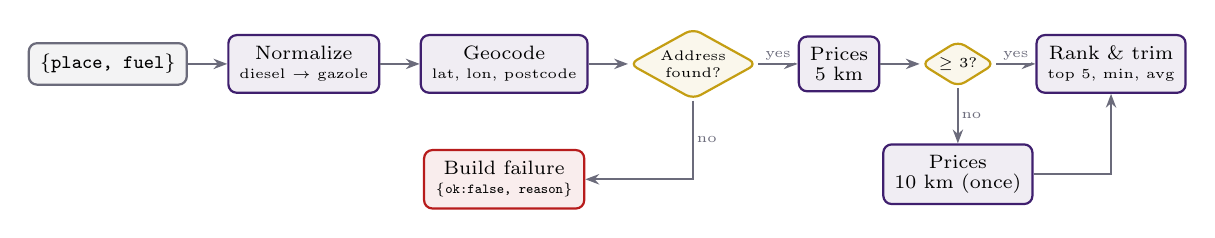
\begin{tikzpicture}[node distance=4mm and 5mm, every node/.style={font=\scriptsize}]
    \node[box=soft] (in) {\ttfamily \{place, fuel\}};
    \node[box, right=of in] (n) {Normalize\\[-1pt]\tiny diesel $\rightarrow$ gazole};
    \node[box, right=of n] (g) {Geocode\\[-1pt]\tiny lat, lon, postcode};
    \node[box=ratzyellow!80!black, diamond, aspect=1.8, inner sep=1pt, right=of g] (f) {\tiny Address\\[-2pt]\tiny found?};
    \node[box, right=of f] (p5) {Prices\\[-1pt]5 km};
    \node[box=ratzyellow!80!black, diamond, aspect=1.6, inner sep=1pt, right=of p5] (e) {\tiny $\geq 3$?};
    \node[box, right=of e] (r) {Rank \& trim\\[-1pt]\tiny top 5, min, avg};
    \node[box, below=7mm of e] (p10) {Prices\\[-1pt]10 km (once)};
    \node[box=rapidored, below=7mm of g] (fail) {Build failure\\[-1pt]\tiny\ttfamily \{ok:false, reason\}};
    \draw[arr] (in) -- (n); \draw[arr] (n) -- (g); \draw[arr] (g) -- (f);
    \draw[arr] (f) -- node[lbl,above]{yes} (p5); \draw[arr] (p5) -- (e);
    \draw[arr] (e) -- node[lbl,above]{yes} (r);
    \draw[arr] (e) -- node[lbl,right]{no} (p10); \draw[arr] (p10) -| (r);
    \draw[arr] (f) |- node[lbl,pos=0.25,right]{no} (fail);
  \end{tikzpicture}

  \vspace{10pt}
  \begin{columns}[T]
    \begin{column}{0.47\textwidth}
      \small
      \begin{itemize}\setlength{\itemsep}{3pt}
        \item \textbf{3 callers, written once}: \cmd{/plein}, the AI agent (as a tool) and the sweep.
        \item The radius widens \textbf{once} to 10\,km when fewer than 3 stations are found.
        \item Field names were \textbf{checked with real API calls} before building the nodes.
      \end{itemize}
    \end{column}
    \begin{column}{0.49\textwidth}
      \small\textbf{Contract}\\[2pt]
      {\ttfamily\scriptsize\color{okgreen}\{ok:true, place\_label, postcode, stations:[top 5], min, avg, spread, radius\_km\}}\\[2pt]
      {\ttfamily\scriptsize\color{rapidored}\{ok:false, reason: place\_not\_found | unknown\_fuel | api\_down\}}\\[3pt]
      {\scriptsize\color{soft}A few hundred bytes, whatever the API returns.}
    \end{column}
  \end{columns}
\end{frame}

% =====================================================================
% 6. WF1
\begin{frame}{WF1 \textperiodcentered{} Rapido: where to fill up}
  \begin{columns}[T]
    \begin{column}{0.56\textwidth}
      \resizebox{\linewidth}{!}{%
      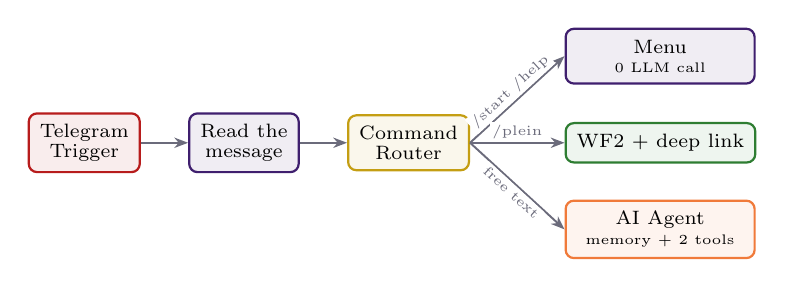
\begin{tikzpicture}[node distance=3.5mm and 6mm]
        \node[box=rapidored] (t) {Telegram\\[-1pt]Trigger};
        \node[box, right=of t] (rm) {Read the\\[-1pt]message};
        \node[box=ratzyellow!80!black, right=of rm] (sw) {Command\\[-1pt]Router};
        \node[box, right=12mm of sw, yshift=11mm, minimum width=2.4cm] (menu) {Menu\\[-1pt]\tiny 0 LLM call};
        \node[box=okgreen, right=12mm of sw, minimum width=2.4cm] (wf2) {WF2 + deep link};
        \node[box=ratzorange, right=12mm of sw, yshift=-11mm, minimum width=2.4cm] (ag) {AI Agent\\[-1pt]\tiny memory + 2 tools};
        \draw[arr] (t) -- (rm); \draw[arr] (rm) -- (sw);
        \draw[arr] (sw.east) -- node[lbl,sloped,above]{/start /help} (menu.west);
        \draw[arr] (sw) -- node[lbl,above]{/plein} (wf2);
        \draw[arr] (sw.east) -- node[lbl,sloped,below]{free text} (ag.west);
      \end{tikzpicture}}
      \vspace{4pt}
      \footnotesize
      \begin{itemize}\setlength{\itemsep}{2pt}
        \item \textbf{AI agent}: NanoGPT model, memory of 10 messages per user.
        \item Tools: \cmd{find\_stations} (WF2) and \cmd{my\_alerts} (alerts table, filtered on the user's \texttt{chat\_id} by the workflow, not by the LLM).
        \item All branches end in \textbf{one} Send node: HTML, split under 4,000 characters.
      \end{itemize}
    \end{column}
    \begin{column}{0.42\textwidth}
      \begin{beamercolorbox}[rounded=true,sep=7pt]{block body}
        \small\textbf{Hand-over to Razmo}\\[3pt]
        \scriptsize Every \cmd{/plein} answer ends with a pre-filled deep link:\\[4pt]
        {\ttfamily\scriptsize t.me/razmo\_carbu\_bot?start=\\\hspace*{1em}\colorbox{ratzyellow!40}{a\_gazole\_222\_94000}}\\[5pt]
        \begin{tabular}{@{}ll@{}}
          \texttt{gazole} & fuel\\
          \texttt{222} & threshold in cents: best price $-$ 3\,c\\
          \texttt{94000} & postcode
        \end{tabular}\\[4pt]
        {\color{soft} Telegram only allows \texttt{[A-Za-z0-9\_-]} in the payload, hence cents and underscores.}
      \end{beamercolorbox}
    \end{column}
  \end{columns}
\end{frame}

% =====================================================================
% 7. WF4
\begin{frame}{WF4 \textperiodcentered{} Razmo: price thresholds}
  \begin{columns}[T]
    \begin{column}{0.55\textwidth}
      \footnotesize\renewcommand{\arraystretch}{1.35}
      \begin{tabular}{@{}>{\raggedright\arraybackslash}p{4.1cm}>{\raggedright\arraybackslash}p{3.7cm}@{}}
        \toprule
        \textbf{Command} & \textbf{What Razmo does}\\
        \midrule
        \cmd{/alerte gazole 1,65 Créteil} & validates, then stores it\\
        \cmd{/start a\_gazole\_165\_94000} & same, from Rapido's link\\
        \cmd{/mesalertes} & numbered list of alerts\\
        \cmd{/stop 2} & deactivates alert n°2\\
        \cmd{/tendance} & lowest price per day, 7 days\\
        \cmd{/sweep} & runs WF3 now (\textbf{owner})\\
        \cmd{/start} & menu; first user = owner\\
        \bottomrule
      \end{tabular}
    \end{column}
    \begin{column}{0.42\textwidth}
      \begin{beamercolorbox}[rounded=true,sep=7pt]{block body}
        \small\textbf{Valid alert?} (If node)\\[3pt]
        \scriptsize
        \faCheck\ known fuel (synonyms normalised)\\
        \faCheck\ threshold between 0.50 and 3.50\eur\\
        \faCheck\ the place geocodes\\[4pt]
        French decimals accepted: \texttt{1,65} $\rightarrow$ 1.65\\[4pt]
        Otherwise Razmo explains \emph{exactly} what is wrong, in character.
      \end{beamercolorbox}
      \vspace{6pt}
      \begin{center}
        \fcolorbox{razmoblue}{razmoblue!6}{\parbox{0.9\linewidth}{\scriptsize\itshape
        ``Razmo a compris. Gazole sous 1,65\eur{} à Créteil. Razmo bouge pas de la pompe.''}}
      \end{center}
    \end{column}
  \end{columns}
\end{frame}

% =====================================================================
% 8. WF3
\begin{frame}{WF3 \textperiodcentered{} Price sweep}
  \centering
  \resizebox{\linewidth}{!}{%
  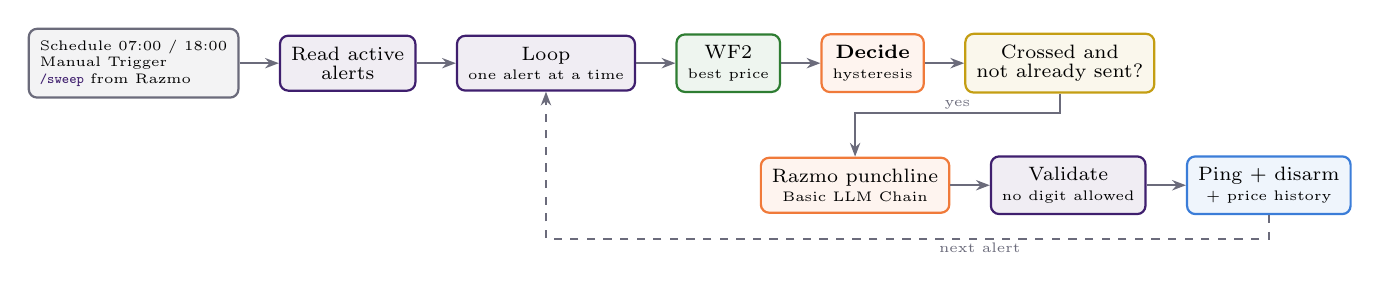
\begin{tikzpicture}[node distance=4mm and 5mm]
    \node[box=soft, align=left] (trg) {\tiny Schedule 07:00 / 18:00\\[-2pt]\tiny Manual Trigger\\[-2pt]\tiny \cmd{/sweep} from Razmo};
    \node[box=ratzpurple, right=of trg] (rd) {Read active\\[-1pt]alerts};
    \node[box, right=of rd] (lp) {Loop\\[-1pt]\tiny one alert at a time};
    \node[box=okgreen, right=of lp] (w2) {WF2\\[-1pt]\tiny best price};
    \node[box=ratzorange, right=of w2] (dc) {\textbf{Decide}\\[-1pt]\tiny hysteresis};
    \node[box=ratzyellow!80!black, right=of dc] (if) {Crossed and\\[-1pt]not already sent?};
    \node[box=ratzorange, below=8mm of if, xshift=-2.6cm] (llm) {Razmo punchline\\[-1pt]\tiny Basic LLM Chain};
    \node[box, right=of llm] (val) {Validate\\[-1pt]\tiny no digit allowed};
    \node[box=razmoblue, right=of val] (ping) {Ping + disarm\\[-1pt]\tiny + price history};
    \draw[arr] (trg) -- (rd); \draw[arr] (rd) -- (lp); \draw[arr] (lp) -- (w2); \draw[arr] (w2) -- (dc); \draw[arr] (dc) -- (if);
    \draw[arr] (if.south) -- ++(0,-0.25) -| node[lbl,pos=0.25,above]{yes} (llm.north);
    \draw[arr] (llm) -- (val); \draw[arr] (val) -- (ping);
    \draw[arr, dashed] (ping.south) -- ++(0,-0.3) -| node[lbl,pos=0.2,below]{next alert} (lp.south);
  \end{tikzpicture}}

  \vspace{12pt}
  \begin{columns}[T]
    \begin{column}{0.48\textwidth}\small
      \begin{itemize}\setlength{\itemsep}{3pt}
        \item One failing alert never blocks the others.
        \item \texttt{price\_history}: one row per place, fuel and am/pm slot (upsert), which feeds \cmd{/tendance}.
      \end{itemize}
    \end{column}
    \begin{column}{0.48\textwidth}\small
      \begin{itemize}\setlength{\itemsep}{3pt}
        \item An alert is disarmed even if Telegram rejects the ping, so it never loops.
        \item \cmd{/sweep} replies with ``N alerts checked, P pings sent''.
      \end{itemize}
    \end{column}
  \end{columns}
\end{frame}

% =====================================================================
% 10. AI with guardrails
\begin{frame}{AI with guardrails: the LLM decides the tone, never the price}
  \begin{columns}[T]
    \begin{column}{0.32\textwidth}
      \centering{\Large\color{ratzorange}\faRobot}\\[2pt]
      \textbf{Where the AI is}\\[4pt]
      \footnotesize\raggedright
      \begin{itemize}\setlength{\itemsep}{2pt}
        \item \rapido's \textbf{AI Agent}: free-text questions, 2 tools, memory
        \item \razmo's \textbf{punchline}: one sentence per ping
      \end{itemize}
      \vspace{6pt}
      \fcolorbox{razmoblue}{razmoblue!6}{\parbox{0.92\linewidth}{\scriptsize\itshape
      Real punchline from the tests:\\ ``Razmo a vu que le gazole devient plus doux pour la bourse et ça lui fait plaisir.''}}
    \end{column}
    \begin{column}{0.32\textwidth}
      \centering{\Large\color{okgreen}\faShield*}\\[2pt]
      \textbf{Guardrails}\\[4pt]
      \footnotesize\raggedright
      \begin{itemize}\setlength{\itemsep}{2pt}
        \item Every price shown is formatted by a \textbf{Code node} from API data
        \item The punchline is \textbf{rejected if it contains a digit} \(\rightarrow\) one of 10 hand-written lines
        \item Agent prompt: ``never a price that does not come from a tool''
      \end{itemize}
    \end{column}
    \begin{column}{0.32\textwidth}
      \centering{\Large\color{razmoblue}\faPlug}\\[2pt]
      \textbf{Provider}\\[4pt]
      \footnotesize\raggedright
      \begin{itemize}\setlength{\itemsep}{2pt}
        \item NanoGPT, \textbf{OpenAI-compatible}: standard OpenAI Chat Model node, only the base URL changes
        \item Tool calling checked with a real call before building the agent
        \item Swapping provider = editing \textbf{one credential}
      \end{itemize}
    \end{column}
  \end{columns}
\end{frame}

% =====================================================================
% 11. Robustness
\begin{frame}{Robustness: both rats keep answering, in character}
  \small\renewcommand{\arraystretch}{1.3}
  \begin{tabular}{@{}p{4.3cm}p{9.6cm}@{}}
    \toprule
    \textbf{When\ldots} & \textbf{\ldots the system} \\
    \midrule
    an API is slow or down & retries 3 times, 2\,s apart, then: \emph{``Les pompes répondent pas à Razmo. Razmo patient.''}\\
    fewer than 3 stations at 5\,km & widens the search to 10\,km, once\\
    the place or fuel is unknown & explains the problem and shows the right syntax\\
    the LLM fails & agent: falls back to \cmd{/plein}, which needs no AI; punchline: template line\\
    the LLM writes a digit & rejects the sentence and uses a template line\\
    a message is too long & splits it under 4,000 characters (Telegram limit)\\
    the sweep runs twice & hysteresis: no duplicate ping; history upsert: no duplicate row\\
    the same \cmd{/alerte} twice & upsert on (chat, fuel, postcode): still one alert\\
    anything crashes & \textbf{WF5} sends the owner the workflow, the node and a link to the run (live test: \cmd{/panne})\\
    \bottomrule
  \end{tabular}
\end{frame}

% =====================================================================
% 12. Stack and credential budget
\begin{frame}{Stack and credential budget}
  \begin{columns}[T]
    \begin{column}{0.48\textwidth}
      \textbf{Only 3 credentials}\\[4pt]
      \small
      \begin{tabular}{@{}ll@{}}
        \toprule
        Telegram Rapido & 1 token, @BotFather \\
        Telegram Razmo & 1 token, same chat \\
        NanoGPT & 1 API key \\
        \midrule
        Fuel-price open data & {\color{okgreen}keyless} \\
        French geocoding API & {\color{okgreen}keyless} \\
        n8n Data Tables & {\color{okgreen}built in} \\
        \bottomrule
      \end{tabular}\\[6pt]
      \scriptsize\color{soft} Avoided on purpose: Google Sheets (OAuth consent screen), hosted Postgres, paid fuel APIs.
    \end{column}
    \begin{column}{0.48\textwidth}
      \textbf{Runtime}\\[4pt]
      \small
      \begin{itemize}\setlength{\itemsep}{3pt}
        \item n8n 2.44.5 in \textbf{Docker Compose}, pinned images, named volume, healthcheck, encryption key from \texttt{.env}
        \item Telegram needs a public HTTPS URL: a free \textbf{Cloudflare tunnel} in a second container
        \item One script, \texttt{start-carbu.sh}: starts the tunnel, reads its URL, starts n8n, re-registers both Telegram webhooks
        \item Same \texttt{chat\_id} in both bots: Rapido can read the alerts stored by Razmo
      \end{itemize}
    \end{column}
  \end{columns}
\end{frame}

% =====================================================================
% 13. Tests
\begin{frame}{Tested before the demo}
  \small
  \begin{columns}[T]
    \begin{column}{0.49\textwidth}
      \begin{itemize}\setlength{\itemsep}{4pt}
        \item[{\color{okgreen}\faCheck}] WF2: real place, nonsense place, synonym (\texttt{diesel}), unknown fuel
        \item[{\color{okgreen}\faCheck}] Hysteresis: test alert at 3.00\eur{}, two sweeps \(\rightarrow\) fired once, then skipped
        \item[{\color{okgreen}\faCheck}] Both parsers on 7 reference inputs, run on the deployed code
      \end{itemize}
    \end{column}
    \begin{column}{0.49\textwidth}
      \begin{itemize}\setlength{\itemsep}{4pt}
        \item[{\color{okgreen}\faCheck}] Every Razmo route and both Rapido routes, end to end
        \item[{\color{okgreen}\faCheck}] The agent calls \cmd{find\_stations(Lyon, gazole)}; its prices match the tool output
        \item[{\color{okgreen}\faCheck}] Telegram webhooks point to the tunnel, 0 errors
      \end{itemize}
    \end{column}
  \end{columns}
  \vfill
  \begin{beamercolorbox}[rounded=true,sep=7pt]{block body}
    \scriptsize\textbf{Bug found, guardrail confirmed.} On the first agent test, the tool failed (``workflow is not active'': a sub-workflow used as an agent tool must be published).
    The agent did \emph{not} invent a price; it answered ``the tool does not respond, try /plein''. WF2 was published and the test passed.
  \end{beamercolorbox}
\end{frame}

% =====================================================================
% 15. Limits, next steps, thanks
\begin{frame}{Known limits and next steps}
  \begin{columns}[T]
    \begin{column}{0.36\textwidth}
      \textbf{Known limits}\\[3pt]
      \scriptsize
      \begin{itemize}\setlength{\itemsep}{2pt}
        \item Agent memory lives in RAM: lost on restart
        \item Free tunnel: the URL changes on restart
        \item Owner = first \cmd{/start}; anyone can message the bots
        \item No brand names in the open data
      \end{itemize}
    \end{column}
    \begin{column}{0.36\textwidth}
      \textbf{Next steps}\\[3pt]
      \scriptsize
      \begin{itemize}\setlength{\itemsep}{2pt}
        \item Group identical alerts: one API call per place and fuel
        \item Telegram location: ``pumps around me''
        \item Persistent memory, allow-listed users
        \item Fixed domain instead of a quick tunnel
      \end{itemize}
    \end{column}
    \begin{column}{0.26\textwidth}
      \centering
      
\includegraphics[height=3.6cm]{img/rapido.png}
    \end{column}
  \end{columns}
\end{frame}

\end{document}
